\documentclass[
    11pt,
    english,
    singlespacing,
    headsepline,
    openany,
]{MastersThesis}

\newcommand{\tabhead}[1]{\textbf{#1}}

\usepackage[utf8]{inputenc} % Required for inputting international characters
\usepackage[T1]{fontenc} % Output font encoding for international characters
\usepackage{mathpazo} % Use the Palatino font by default

\usepackage[backend=bibtex,style=authoryear,natbib=true]{biblatex} % Use the bibtex backend with the authoryear citation style (which resembles APA)

\addbibresource{refs.bib} % The filename of the bibliography

\usepackage[autostyle=true]{csquotes} % Required to generate language-dependent quotes in the bibliography

\usepackage{amsmath}
\usepackage[linesnumbered,ruled,vlined]{algorithm2e}
\usepackage{svg}
%----------------------------------------------------------------------------------------
%	MARGIN SETTINGS
%----------------------------------------------------------------------------------------

\geometry{
	paper=a4paper, % Change to letterpaper for US letter
	inner=2.5cm, % Inner margin
	outer=3.8cm, % Outer margin
	bindingoffset=.5cm, % Binding offset
	top=1.5cm, % Top margin
	bottom=1.5cm, % Bottom margin
	%showframe, % Uncomment to show how the type block is set on the page
}

%----------------------------------------------------------------------------------------
%	THESIS INFORMATION
%----------------------------------------------------------------------------------------

\thesistitle{Point cloud human pose estimation using capsule networks}
\supervisor{Andrii \textsc{Babii}}
\degree{Master of Science}
\author{Oleksandr \textsc{Onbysh}}

\subject{Data Science}
\keywords{}
\university{\href{http://www.ucu.edu.ua}{Ukrainian Catholic University}}
\department{\href{http://department.university.com}{Faculty of Applied Sciences}}
\group{\href{http://researchgroup.university.com}{Department of Computer Sciences}}
\faculty{\href{http://faculty.university.com}{}}

\begin{document}

\frontmatter 
\pagestyle{plain} 

%----------------------------------------------------------------------------------------
%	TITLE PAGE
%----------------------------------------------------------------------------------------

\begin{titlepage}
\begin{center}

\vspace*{.06\textheight}
{\scshape\LARGE \univname\par}\vspace{1.5cm} % University name
\textsc{\Large Master Thesis}\\[0.5cm] % Thesis type

\HRule \\[0.4cm] % Horizontal line
{\huge \bfseries \ttitle\par}\vspace{0.4cm} % Thesis title
\HRule \\[1.5cm] % Horizontal line
 
\begin{minipage}[t]{0.4\textwidth}
\begin{flushleft} \large
\emph{Author:}\\
\href{https://www.linkedin.com/in/alexanderonbysh/}{\authorname}
\end{flushleft}
\end{minipage}
\begin{minipage}[t]{0.4\textwidth}
\begin{flushright} \large
\emph{Supervisor:} \\
\href{https://nure.ua/en/staff/andrii-babii}{\supname}
\end{flushright}
\end{minipage}\\[3cm]
 
\vfill

\large \textit{A thesis submitted in fulfillment of the requirements\\ for the degree of \degreename}\\[0.3cm] % University requirement text
\textit{in the}\\[0.4cm]
\groupname\\\deptname\\[2cm]
 
\vfill
\includegraphics[scale=0.15]{logo.png} % University/department logo - uncomment to place it

\vfill
{\large Lviv 2021}\\[4cm] % Date

\end{center}
\end{titlepage}

%----------------------------------------------------------------------------------------
%	DECLARATION PAGE
%----------------------------------------------------------------------------------------

\begin{declaration}
\addchaptertocentry{\authorshipname} % Add the declaration to the table of contents
\noindent I, \authorname, declare that this thesis titled, \enquote{\ttitle} and the work presented in it are my own. I confirm that:

\begin{itemize} 
\item This work was done wholly or mainly while in candidature for a research degree at this University.
\item Where any part of this thesis has previously been submitted for a degree or any other qualification at this University or any other institution, this has been clearly stated.
\item Where I have consulted the published work of others, this is always clearly attributed.
\item Where I have quoted from the work of others, the source is always given. With the exception of such quotations, this thesis is entirely my own work.
\item I have acknowledged all main sources of help.
\item Where the thesis is based on work done by myself jointly with others, I have made clear exactly what was done by others and what I have contributed myself.
\end{itemize}
 
\noindent Signed:\\
\rule[0.5em]{25em}{0.5pt} % This prints a line for the signature
 
\noindent Date:\\
\rule[0.5em]{25em}{0.5pt} % This prints a line to write the date
\end{declaration}

\cleardoublepage

%----------------------------------------------------------------------------------------
%	QUOTATION PAGE
%----------------------------------------------------------------------------------------

\vspace*{0.2\textheight}

\noindent\enquote{\itshape Thanks to my solid academic training, today I can write hundreds of words on virtually any topic without possessing a shred of information, which is how I got a good job in journalism.}\bigbreak

\hfill Dave Barry

%----------------------------------------------------------------------------------------
%	ABSTRACT PAGE
%----------------------------------------------------------------------------------------

\begin{abstract}
\addchaptertocentry{\abstractname} % Add the abstract to the table of contents
Human pose estimation based on points cloud is an emerging field that develops with 3D scanning devices' popularity. Build-in LiDAR technology in mobile phones and a growing VR market creates a demand for lightweight and accurate models for 3D point cloud. Widely advanced deep learning tools are mainly used for structured data, and they face new challenges in unstructured 3D space. Recent research on capsule networks proves that this type of model outperforms classical CNN architectures in tasks that require viewpoint invariance from the model. Thus capsule networks challenge multiple issues of classic CNNs like preserving the orientation and spatial relationship of extracted features, which could significantly improve the 3D points cloud classification task's performance.

The project's objective is to experimentally assess the applicability of capsule neural network architecture to the task of point cloud human pose estimation and measure performance on non-synthetic data. Additionally, measure noise sustainability of capsule networks for 3D data compared to regular models. Compare models' performance with restricted amount of training data.
\end{abstract}

%----------------------------------------------------------------------------------------
%	ACKNOWLEDGEMENTS
%----------------------------------------------------------------------------------------

\begin{acknowledgements}
\addchaptertocentry{\acknowledgementname} % Add the acknowledgements to the table of contents
The acknowledgments and the people to thank go here, don't forget to include your project advisor\ldots
\end{acknowledgements}

%----------------------------------------------------------------------------------------
%	LIST OF CONTENTS/FIGURES/TABLES PAGES
%----------------------------------------------------------------------------------------

\tableofcontents % Prints the main table of contents
\listoffigures % Prints the list of figures
\listoftables % Prints the list of tables

%----------------------------------------------------------------------------------------
%	ABBREVIATIONS
%----------------------------------------------------------------------------------------

\begin{abbreviations}{ll} % Include a list of abbreviations (a table of two columns)

\textbf{CapsNet} & Capsule network \\


\end{abbreviations}

%----------------------------------------------------------------------------------------
%	SYMBOLS
%----------------------------------------------------------------------------------------

\begin{symbols}{lll} % Include a list of Symbols (a three column table)


$P$ & set of points in $D$ space (point cloud) \\
$J$ & set of key joints positions \\
$N$ & resolution of point cloud (number of points in one cloud) \\


% \addlinespace % Gap to separate the Roman symbols from the Greek
\end{symbols}

%----------------------------------------------------------------------------------------
%	THESIS CONTENT - CHAPTERS
%----------------------------------------------------------------------------------------

\mainmatter % Begin numeric (1,2,3...) page numbering

\pagestyle{thesis} % Return the page headers back to the "thesis" style

% Include the chapters of the thesis as separate files from the Chapters folder
% Uncomment the lines as you write the chapters

% Chapter Template

\chapter{Introduction} % Main chapter title

\label{Introduction}


\section{Problem}
Human pose estimation is a task based on a human's image or 3D points, and the model should locate the main joints in the human's body (head, neck, left and right arms, spin, etc.) as shown in the Figure  \ref{example}. Each joint is represented as a point in 2D or 3D space based on the task's objective.

\begin{figure}[htbp]
\centerline{\includegraphics[scale=.5]{Figures/introduction-einstein.png}}
\caption{Example of human pose estimation key points \cite{rovai_realtime_2020}}
\label{example}
\end{figure}

A 3D point cloud is simply a set of points with three positional coordinates and represents points in 3D space. The points represent the shape of the object in 3D space. 3D point clouds are usually gathered by 3D scanners or dual-lens cameras.The output of scanners is point cloud where each point corresponds to some point on scanning surface with predefined precision. With the rapid growth of LIDAR and VR fields, the importance of accurate and fast 3D point cloud human pose estimation algorithms is clear.

\section{Challenges}
The obvious challenge of human pose estimation is the potential space of different human postures. The small change in the body part position changing the target pose. The task gets more complicated with different obstacles like clothes.
Using recent ML algorithms such as deep learning on 3D point cloud results in many challenges. Some of the common issues are:
\begin{itemize}
  \item The high dimensionality of the input space. Compared to pose estimation based on images, 3D point cloud has higher-dimensional space.
  \item Noisy inputs from 3D point cloud scanners. The sparsity and accuracy of the point cloud greatly influence the model's performance. The accuracy and granularity of points are significantly dependent on the scanning device. Compact LIDAR scanning devices the most popular and less accurate.
  \item Geometric-viewpoint relation. The human body has a strict geometric relation between body parts, which is invariant to the viewpoint. Most of the deep learning algorithms are not viewpoint agnostic resulting in additional challenges for human pose estimation.
  \item Lack of data. The amount of data for 3D point cloud human pose estimation is significantly less than regular image datasets. This fact is due to the high complexity of collecting 3D point cloud data, e.g., need special multicamera or LIDAR equipment, need diverse human positions, need different human constitutions.
\end{itemize}

\section{Motivation}
Human pose estimation is an important task that is used in different fields.
A recent class of deep learning architecture known as capsule networks \cite{sabour_dynamic_2017} theoretically overcomes multiple conventional deep learning models for human pose estimation. Compared to CNNs, capsule networks, due to the dynamic routing algorithm, account for the spatial relation between the input scene parts. Additionally, capsule networks "learn" the object's geometric relationship and thus could be viewpoint agnostic \cite{sabour_dynamic_2017}. These capsule networks' properties make them the right candidate for examining human pose estimators based on the point cloud.
Moreover, some experiments stated that capsule networks need less data for convergence compared to non-capsule models. Besides, due to latent space inside the capsule network, it is more noise agnostic than regular convolutional networks.

\section{Research Gap}
\begin{itemize}
  \item There is no capsule-based model for 3D human pose estimation task.
  \item Compare the influence of noisy data on capsule-based and non-capsule-based models.
  \item Compare convergence of capsule-based and non-capsule based models with the truncated training dataset.
\end{itemize}

\section{Objective}
The work's objective is to propose a model based on a capsule network for a 3D point cloud human pose estimation. Evaluate the model on public benchmark datasets for human pose estimation. Compare results with state of the art approaches for the task as mentioned earlier. Evaluate the influence of the noise in training dataset on capsule-based and non-capsule-based networks. Measure the convergence speed of the models with different sizes of training dataset.

\section{Paper structure}
Section \ref{releated work} covers the related work of human pose estimation based on both 2D images and 3D point clouds. This section described conventionally, and state of the art approaches for solving the issue. Reviews capsule networks for different 3D point cloud tasks like point classification, segmentation, and position estimation.

The rest of the paper is organized in the following manner:
% TODO: fill with sections
\begin{itemize}
  \item Section \ref{hypothesis} presents the project's hypothesis and problems;
  \item  section \ref{approach} describes the approach for solving the project's objection and provide timelines;
  \item  section \ref{conclusion} sums up the paper's ideas and present brief conclusions and possible future work in this field.
\end{itemize}
\chapter{Related work}

\label{Related work}

\section{Deep learning approaches for point cloud}
The different number of points and high dimensionality of the point cloud input makes it challenging to use regular 2D convolutions. The typical approach for such an issue is the conversation of the point cloud to a different format. Such approaches are projection-based methods, volumetric-based methods, and other geometric based methods.
\subsection{Projection-based methods} take point cloud and project it into a different panel view. After the projection, each view provides a set of combined features for target classification, regression, or segmentation. The critical challenge for the projection-based algorithm is the multi-view feature aggregation into one global feature space.
MVCNN \parencite{su_multi-view_2015} is the first model that presents a standard CNN architecture trained to recognize the shapes' rendered views independently of each other and show that a 3D shape can be recognized even from a single view at an appropriate accuracy. Recognition rates further increase when multiple views of the shapes are provided.
MHBN \parencite{yu_multi-view_2018} (Multi-view Harmonized Bilinear Network) is the continuation of MVCNN. The approach proposes to integrates local convolutional features by harmonized bilinear pooling to produce a compact global descriptor.
To persist the information from different views, the View-GCN \parencite{wei_view-gcn_2020} proposes constructing view-graph with multiple views as graph nodes, then designing a graph convolutional neural network over view-graph to learn discriminative shape descriptor hierarchically.
All projection-based methods struggle from high memory consumption and high computational complexity since, for one feature extraction, the model should be run for the number of different views.

\subsection{Volumetric-based methods} map the point cloud into a 3D grid. Then conventional 3D convolutions are using for feature extraction.
VoxNet \parencite{maturana_voxnet_2015} is the first method that exploits the volumetric representation of the point cloud. In this work, each cloud point is mapped to a discrete voxel point. The size of the target grid is 32 x 32 x 32 voxels. After the mapping, three convolutional layers are using to produce the target feature representations.
The more advanced volumetric-based models use octrees data structure. OctNet \parencite{riegler_octnet_2017} propose to represent the point cloud as several octrees along a regular grid, each octree is encoded as a bit string, and features are generated through naive arithmetic. This approach reduces the memory consumption of the model during the training and inference stages.
The next iteration of octrees representation of point cloud is proposed in O-CNN \parencite{wang_o-cnn_2017}. The model uses 3D convolutions to extract features from octrees. Built upon the octree representation of 3D shapes, the method takes the average normal vectors of a 3D model sampled in the finest leaf octants as input and performs 3D CNN operations on the octants occupied by the 3D shape surface.

\section{Point-based Methods}
Compared with projection-based methods and volumetric-based methods that aggregate points from a spatial neighborhood, point-based methods attempt to learn features from individual points. Most of the recent work focuses on this direction.

The first work which use point-based approach is PointNet \parencite{qi_pointnet_2017}. PointNet learns pointwise features independently with several MLP layers and extracts global features with a max-pooling layer. The input (an $n \times 3$ 2D tensor) is first multiplied by an affine transformation matrix predicted by a mini-network (T-Net) to hold invariance under geometric transformations. The point set is then passed through a group of MLPs followed by another joint alignment network, and a max-pooling layer to obtain the final global feature.

The second iteration of PointNet is PointNet++ \parencite{qi_pointnet_2017-1}. PointNet++ introduce a hierarchical neural network that applies PointNet recursively on a nested partitioning of the input point set. By exploiting metric space distances, network is able to learn local features with increasing contextual scales.

The state of the art model for point-based classification is Point Attention Transformers \parencite{yang_modeling_2019}. The research for the first time propose an end-to-end learnable and taskagnostic sampling operation, named Gumbel Subset Sampling (GSS), to select a representative subset of input points. Equipped with Gumbel-Softmax, it produces a ”soft” continuous subset in training phase, and a ”hard” discrete subset in test phase. By selecting representative subsets in a hierarchical fashion, the networks learn a stronger representation of the input sets with lower computation cost.

\section{Human pose estimation}
The latest research approaches in the field of human pose estimation are based on deep learning.
There are two main approaches to the task:
\begin{itemize}
  \item pose estimation based on 2D images (mostly RGB);
  \item pose estimation based on the 3D point cloud.
\end{itemize}

The latter approach is more recent and promising. The 3D perspective gives more information for the models about body position in the space. Also, 3D point clouds mitigate the issue with occluded parts of the body. 2D image is a 2D projection of 3D space, and this transformation leads to the loss of information.

\subsection{Image-based methods}
The approaches for 2D image human pose estimation are devided into two types:
\begin{itemize}
  \item top-down approach
  \item bottom-up approach
\end{itemize}
In the top-down approach the first step is person detection and then pose regression. In bottom-up approach all body parts are detected first, and then grouped according to body's position.

OpenPose \parencite{cao_openpose_2019} is the most popular example of bottom-up approaches for multi-person pose estimation. The network first extracts features from the image using VGG feature extractor. Then features are passed to two separate branches, first branch predicts body parts key points, second branch predict the associativity between body parts.

RMPE (AlphaPose) \parencite{fang_rmpe_2018} is a top-down model. This approach propose to use Symmetric Spatial Transformer Network (SSTN) to extract person regions based on bounding boxes. A Single Person Pose Estimator (SPPE) is used in this extracted region to estimate the human pose skeleton for that person. A Spatial De-Transformer Network (SDTN) is used to remap the estimated human pose back to the original image coordinate system. Finally, a parametric pose Non-Maximum Suppression (NMS) technique is used to handle the issue of redundant pose deductions.

\subsection{point-cloud-based methods}. Point cloud based estimation is relatively young field due to recent growth of popularity of point cloud scanning devices.

The first model for human pose estimation based on point cloud is \parencite{diaz_barros_real-time_2015}. The paper presents an approach where based on predefined human body skeleton the input point cloud is clustered using PCA and Expectation maximization algorithms.

The recent work in this field is presented in \parencite{zhou_learning_2020}. Paper propose a deep human pose network for 3D pose estimation by taking the point cloud data as input data to model the surface of complex human structures. This approach is end to end, first cast the 3D human pose estimation from 2D depth images to 3D point clouds and directly predict the 3D joint position.

More point cloud human pose estimation methods will be covered in the next subsection. Next subsection covers models which are based on capsule architecture.

\section{Capsule network}
The concept of the capsule was first proposed by Hinton \parencite{sabour_dynamic_2017} and has been widely used in 2D and 3D deep learning \parencite{kakillioglu_3d_2020, qin_detecting_2020, duarte_videocapsulenet_2018, lalonde_capsules_2018}.

Capsules represents as a set of vectors. The length of the capsule's vector represents the probability of the object's presence. Direction of the vector describes object's property e.g. position, viewpoint, size, shape, etc. For capsules' training Hinton propose a new algorithm \parencite{sabour_dynamic_2017} called dynamic routing. The forward pass with dynamic routing propagate the input data from lower level capsules to higher level ones. Lower level capsules pass learned and predicted data to the higher level capsules. If multiple lower-level capsules agrees (activated) then higher-level capsules activates accordingly. With each iteration of dynamic routing each capsules gets more accurate.

\subsection{Capsule networks for point cloud classification}. The first work where capsule networks were applied to the problem of point cloud classification is 3DCapsNet \parencite{cheraghian_3dcapsule_2018}. In this work a new capsule-based layer is proposed - ComposeCaps. ComposeCaps learns spatially relevant feature mapping that can be exploited for 3D point cloud classification.
The second iteration of capsule applicability to 3D classification is 3D point capsule network \parencite{zhao_3d_2019}. 3D point capsule network is an auto-encoder designed based on capsule networks. In this work researchers propose new architecture with capsule network encoder which encode input point cloud to capsules' latent space, and decoder which decode latent capsules. The proposed architecture works for several common point cloud-related tasks, such as object classification, object reconstruction and part segmentation.

\subsection{Capsule networks for point cloud regression.} The only work which is currently presented on the topic of point cloud regression is Capsule-HandsNet \parencite{wu_3d_2020}. This project is inspired by this research. Capsule-HandsNet proposes an end-to-end capsule-based hand pose estimation network, which processes hand point clouds directly with the consideration of structural relationships among local parts, including symmetry, junction, relative location, etc.The model works in autoencoder maner the same as in \parencite{zhao_3d_2019}.
 
\chapter{Research Hypothesis and Problem}

\label{Hypothesis}

\section{Hypotheses}
\paragraph{Model Comparison hypothesis:} This project's main objective is to create a model for human pose estimation based on point cloud using a capsule-based neural network, which shows competitive accuracy on well-known benchmarks.

\paragraph{Noise resistance hypothesis:} the impact of noise in the training dataset on the capsule-based model should be less compared to non-capsule models. Hypothesis is made based on 2D image recognition based using capsule networks \cite{sabour_dynamic_2017}.
Dataset size hypothesis: The dataset's size for full convergence should be smaller for capsule-based network compared to non-capsule ones. Assumption is made based on experiments presented in \cite{sabour_dynamic_2017} based on 2D image classification.

\section{Problems}
\paragraph{Noise problem.} To achieve the project goal mentioned above, we need to create an algorithm that could create realistic noise for point cloud data. We need to analyze and replicate factors that influence scanning devices' accuracy and result in noisy data.
\paragraph{Models' retrain problem.} To achieve the project's third goal, we need to retrain reference sota models with truncated training data. Hence, we need to allocate additional time for such an activity.
\chapter{Methodology}
\label{Methodology}

In this section we introduce the methodology for our proposed method for the task of human pose estimation using point cloud. As we reviewed in \ref{Related work} the key issue of any which use point clouds as an input is huge spatial variation of the data. Point clouds much diverse compared to 2D images in terms of location and rotation. Capsule networks shows promising results \parencite{sabour_dynamic_2017} on 2D data, and better handle spatial invariance compared to regular NN models.  \\
The chapter consists of two main section. In \ref{Data preparation} section we will cover the preprocessing for the input data and ground truths, and methods of adding artificial noise the the input data. In \ref{Network architecture} we will cover the network's architecture and algorithms for performing network's training.


\section{Data preparation}
\label{Data preparation}
In this section we will cover main preprocessing steps for datasets. Preprocessing consists of:
\begin{enumerate}
  \item human extraction;
  \begin{enumerate}
    \item threshold filtering;
    \item clusterization \& cluster selection;
  \end{enumerate}
  \item point cloud normalization;
  \item adding noise to data (optional).
\end{enumerate}

On the first step we remove the most obvious points which doesn't represent human posture. On the second step we perform segmentation to extract "human" cluster. The third step is optional, and is used in experiments with performance of different models with various levels of the noise.


\subsection{Human extraction}
To start working with points cloud for human pose estimation we decided to extract human human points out of overall point cloud. As we can see from the Figure \ref{img:example-of-raw-data}, the raw point cloud contains not only human point cloud but also other objects which are located in the room, such as walls, cupboards, and other objects. These obstacles will not only harm the model's performance but will also greatly slow down the model's training and inference due to excess number of point.

\begin{figure}[htbp]
    \centerline{\includegraphics[scale=.4]{Figures/template.png}}
    \caption{Example of raw data from ITOP dataset (front view)}
    \label{img:example-of-raw-data}
\end{figure}

\subsubsection{Threshold filtering}
\label{s:threshold-filtering}
Threshold filtering is the first step in preprocessing pipeline. The aim of this step is to filter out the most obvious points which don't belong to the human posture.
After manual checks we came up to such parameters:  

\begin{equation}
    \begin{aligned}
        x_{min} &= -1   &x_{max} &= 1 \\
        y_{min} &= -1.4 &y_{max} &= 2 \\
        z_{min} &= -1.5 &z_{max} &= 3.5
    \end{aligned}
\label{eqn:threshold-values}
\end{equation}

\ref{eqn:threshold-values} sets min-max distance values from camera view. The camera sensor is considered as center - $(0, 0, 0)$. In this way, $x$ coordinate represents left-right direction from the camera center, $y$ - top-bottom, and $z$ - the depth. \\
An example of threshold filtered point cloud could be seen in Figure~\ref{img:after-threshold-filtering}.

\begin{figure}[htbp]
    \centerline{\includegraphics[scale=.4]{Figures/template.png}}
    \caption{Example of point cloud after applying of threshold filter}
    \label{img:after-threshold-filtering}
\end{figure}

\subsubsection{Clusterization}
The next step in preprocessing is clusterization \& extraction. On this step we clusterize point cloud from the \ref{s:threshold-filtering} and extract the human cluster. For clusterization step we propose the nearest-neighbour search algorithm \parencite{noauthor_nearest_2021} with kd-tree data-structure, using FLANN \footnote{Fast Library for Approximate Nearest Neighbor}. \\
The aim of the clusterization is separate human cluster and small noisy clusters from the point cloud. As we can see from the Algorithm~\ref{alg:clusterization}, for each point in initial point cloud $P$ we try to put it to some cluster based on the distance (radius - $r$) of that cluster. If the distance is less that radius to each cluster then this point creates a new cluster. At the end of clusterization we get a set of clusters $C$. \\
Since the human cluster always the biggest, at the end of clusterization we take the argmax and get human cluster $C_{human}$.

On the Figure~\ref{img:after-clustering} we can see the point cloud before clusterization, after, and the resulting human cluster (the biggest cluster). \\

\begin{algorithm}[H]
\label{alg:clusterization}
\SetAlgoLined
\KwResult{human point cloud cluster - $C_{human}$}
 create a Kd-tree representation for the input point cloud dataset $P$ \;
 set up an empty list of clusters $C$, and a queue of the points that need to be checked $Q$ \;
\For{\texttt{every point} $p_i \in P$} {
    add $p_i$ to the current queue $Q$ \;
    \For{\texttt{every point} $p_i \in Q$}{
        search for the set $P^k_i$ of point neighbors of $p_i$ in a sphere with radius $r < d_{th}$ \;
        for every neighbor $p^k_i \in P^k_i$, check if the point has already been processed, and if not add it to $Q$\;
    }
    when the list of all points in $Q$ has been processed, add $Q$ to the list of clusters $C$, and reset $Q$ to an empty list \;
}
the algorithm terminates when all points $\boldsymbol{p}_i \in P$ have been processed and are now part of the list of point clusters $C$ \;
$C_{human} = \underset{ x \in C }{\arg\max}$

\caption{Point cloud clusterization and human extraction \parencite{noauthor_pcl_nodate}}
\end{algorithm}

\begin{figure}[htbp]
    \centerline{\includegraphics[scale=.4]{Figures/template.png}}
    \caption{Example of point cloud after applying of threshold filter}
    \label{img:after-clustering}
\end{figure}

\subsection{Point cloud normalization}
TBD



\subsection{Adding noise to data}
Noise is the common thing in point cloud data. The origin the the noise could be environment conditions such as dust, fog, and other particles in the air. Also, the noise appears due to unperfectness on the lidar and other tools of creating point clouds.

In Experiment~\ref{s:experiment-noise} we investigate how models perform with different amount of artificial noise in the input data. For that we need to generate the noise which could be similar to the real-world. We propose to use two types of noise:
\begin{itemize}
  \item Gaussian noise;
  \item outlier noise.
\end{itemize}

\subsubsection{Gaussian noise}
The Gaussian noise is adding noise to the initial points in the point cloud $P$. With probability of $p$ the Gaussian noise ($\sigma$, $\mu$) is added to the point $p \in P$. In this way we simulate the unperfectness of the detecting device. The generation process is described in Algorithm~\ref{alg:gaussian-noise}

\begin{algorithm}[H]
\label{alg:gaussian-noise}
\SetAlgoLined
\KwResult{human point cloud with Gaussian noise  - $\hat{P_{human}}$}
\For{\texttt{every point} $p_i \in P$} {
    \If{ \texttt{uniRand()} < $Prob_{noise}$ } {
        Set $p_x$ to $p_x$ + $Gaus(\sigma, \mu)$ \;
        Set $p_y$ to $p_y$ + $Gaus(\sigma, \mu)$ \;
        Set $p_z$ to $p_z$ + $Gaus(\sigma, \mu)$ \;
    }
}
\caption{Adding Gaussian noise to point cloud \parencite{uchida_tom-uchidaadd_noise_to_point_cloud_2021}}
\end{algorithm}

An example of applying the Gaussian noise to the point cloud could be seen in the Figure~\ref{img:gaussian-noise}

\begin{figure}[htbp]
    \centerline{\includegraphics[scale=.6]{Figures/coords_gaussian.png}}
    \caption{Example of pllying the Gaussian noise to the point cloud \parencite{uchida_tom-uchidaadd_noise_to_point_cloud_2021}}
    \label{img:gaussian-noise}
\end{figure}

\subsubsection{Outlier noise}
The outlier noise adding new points to the initial point cloud $P$. The amount of outlier noise is defined by the fraction of the noise points compared to the initial number of human points. The noise point is taken from the uniform distribution $U(a, b)$. Where $a$ and $b$ are min-max values from the initial point cloud. In this way, outlier noise will fill uniformly the bounding box of the initial point cloud.

An example of addition of the outlier noise to the point cloud could be seen in the Figure~\ref{img:outlier-noise}

\begin{figure}[htbp]
    \centerline{\includegraphics[scale=.6]{Figures/coords_outlier.png}}
    \caption{Example of addition the outlier noise to the point cloud \parencite{uchida_tom-uchidaadd_noise_to_point_cloud_2021}}
    \label{img:outlier-noise}
\end{figure}

\section{Network architecture}
\label{Network architecture}
\subsection{Capsule network autoencoder}
\subsubsection{Chamfer distance}
\subsection{Capsule-based regression network}

\section{Network training}

 
\chapter{Dataset and evaluation metrics}
\label{Dataset}

In the first section (\ref{dataset}) we describe the dataset which is used for training and evaluation purpose for the task of the human pose estimation.
In the second (\ref{evaluation-metric}) section the define the evaluation metric for aforementioned

\section{Dataset}
The most common datasets for the task of human pose estimation from point clouds are ITOP \parencite{haque_towards_2016} and EVAL \parencite{liu_point_2020}. In this work we concentrate on ITOP dataset since it's more widely used thus has more related works for results' comparison.

\label{dataset}
\subsection{ITOP}

ITOP dataset was first released in the work of \cite{haque_towards_2016}. The dataset comprises depth images of people in different poses. In Figure~\ref{img:dataset-points-with-depth} are shown example of the depth map from the dataset. 

The snapshots of poses are taken from two different viewpoints: the front view, and the top view. In front view the camera faces a person directly in front (the whole body is seen). In top view the camera is placed above the person and shots the view from the top (torso usually occluded by shoulders and arms).

The dataset is collected inside of the room thus some furniture items appear in the dataset. Due to excess obstacles in the field of view of the camera, we apply preprocessing pipelines to extract only human point cloud. The pipeline is described in Section~\ref{Data-preparation}. Figures \ref{img:dataset-human-examples-front-view} and \ref{img:dataset-human-examples-top-view} show examples of font and top view respectively.

Ground truths consist of 15 joint key points - head, neck, shoulders, elbows, hands, torso, hips, knees, and foots. An example of named joints is shown in Figure~\ref{img:dataset-example-joints}. Table~\ref{tab:dataset-statistic} covers general statistics on dataset size.

\begin{table}
    \label{tab:dataset-statistics}
    \caption{General statistic for ITOP dataset}
    \centering
    \begin{tabular}{l l l l}
    \toprule
    \tabhead{View} & \tabhead{Split} & \tabhead{Frames} & \tabhead{People} \\
    \midrule
        side & train & 39,795 & 16 \\
        side & test  & 10,501 & 4  \\
        top  & train & 39,795 & 16 \\
        top  & test  & 10,501 & 4  \\
    \bottomrule\\
    \end{tabular}
\end{table}

\begin{figure}[htbp]
    \centerline{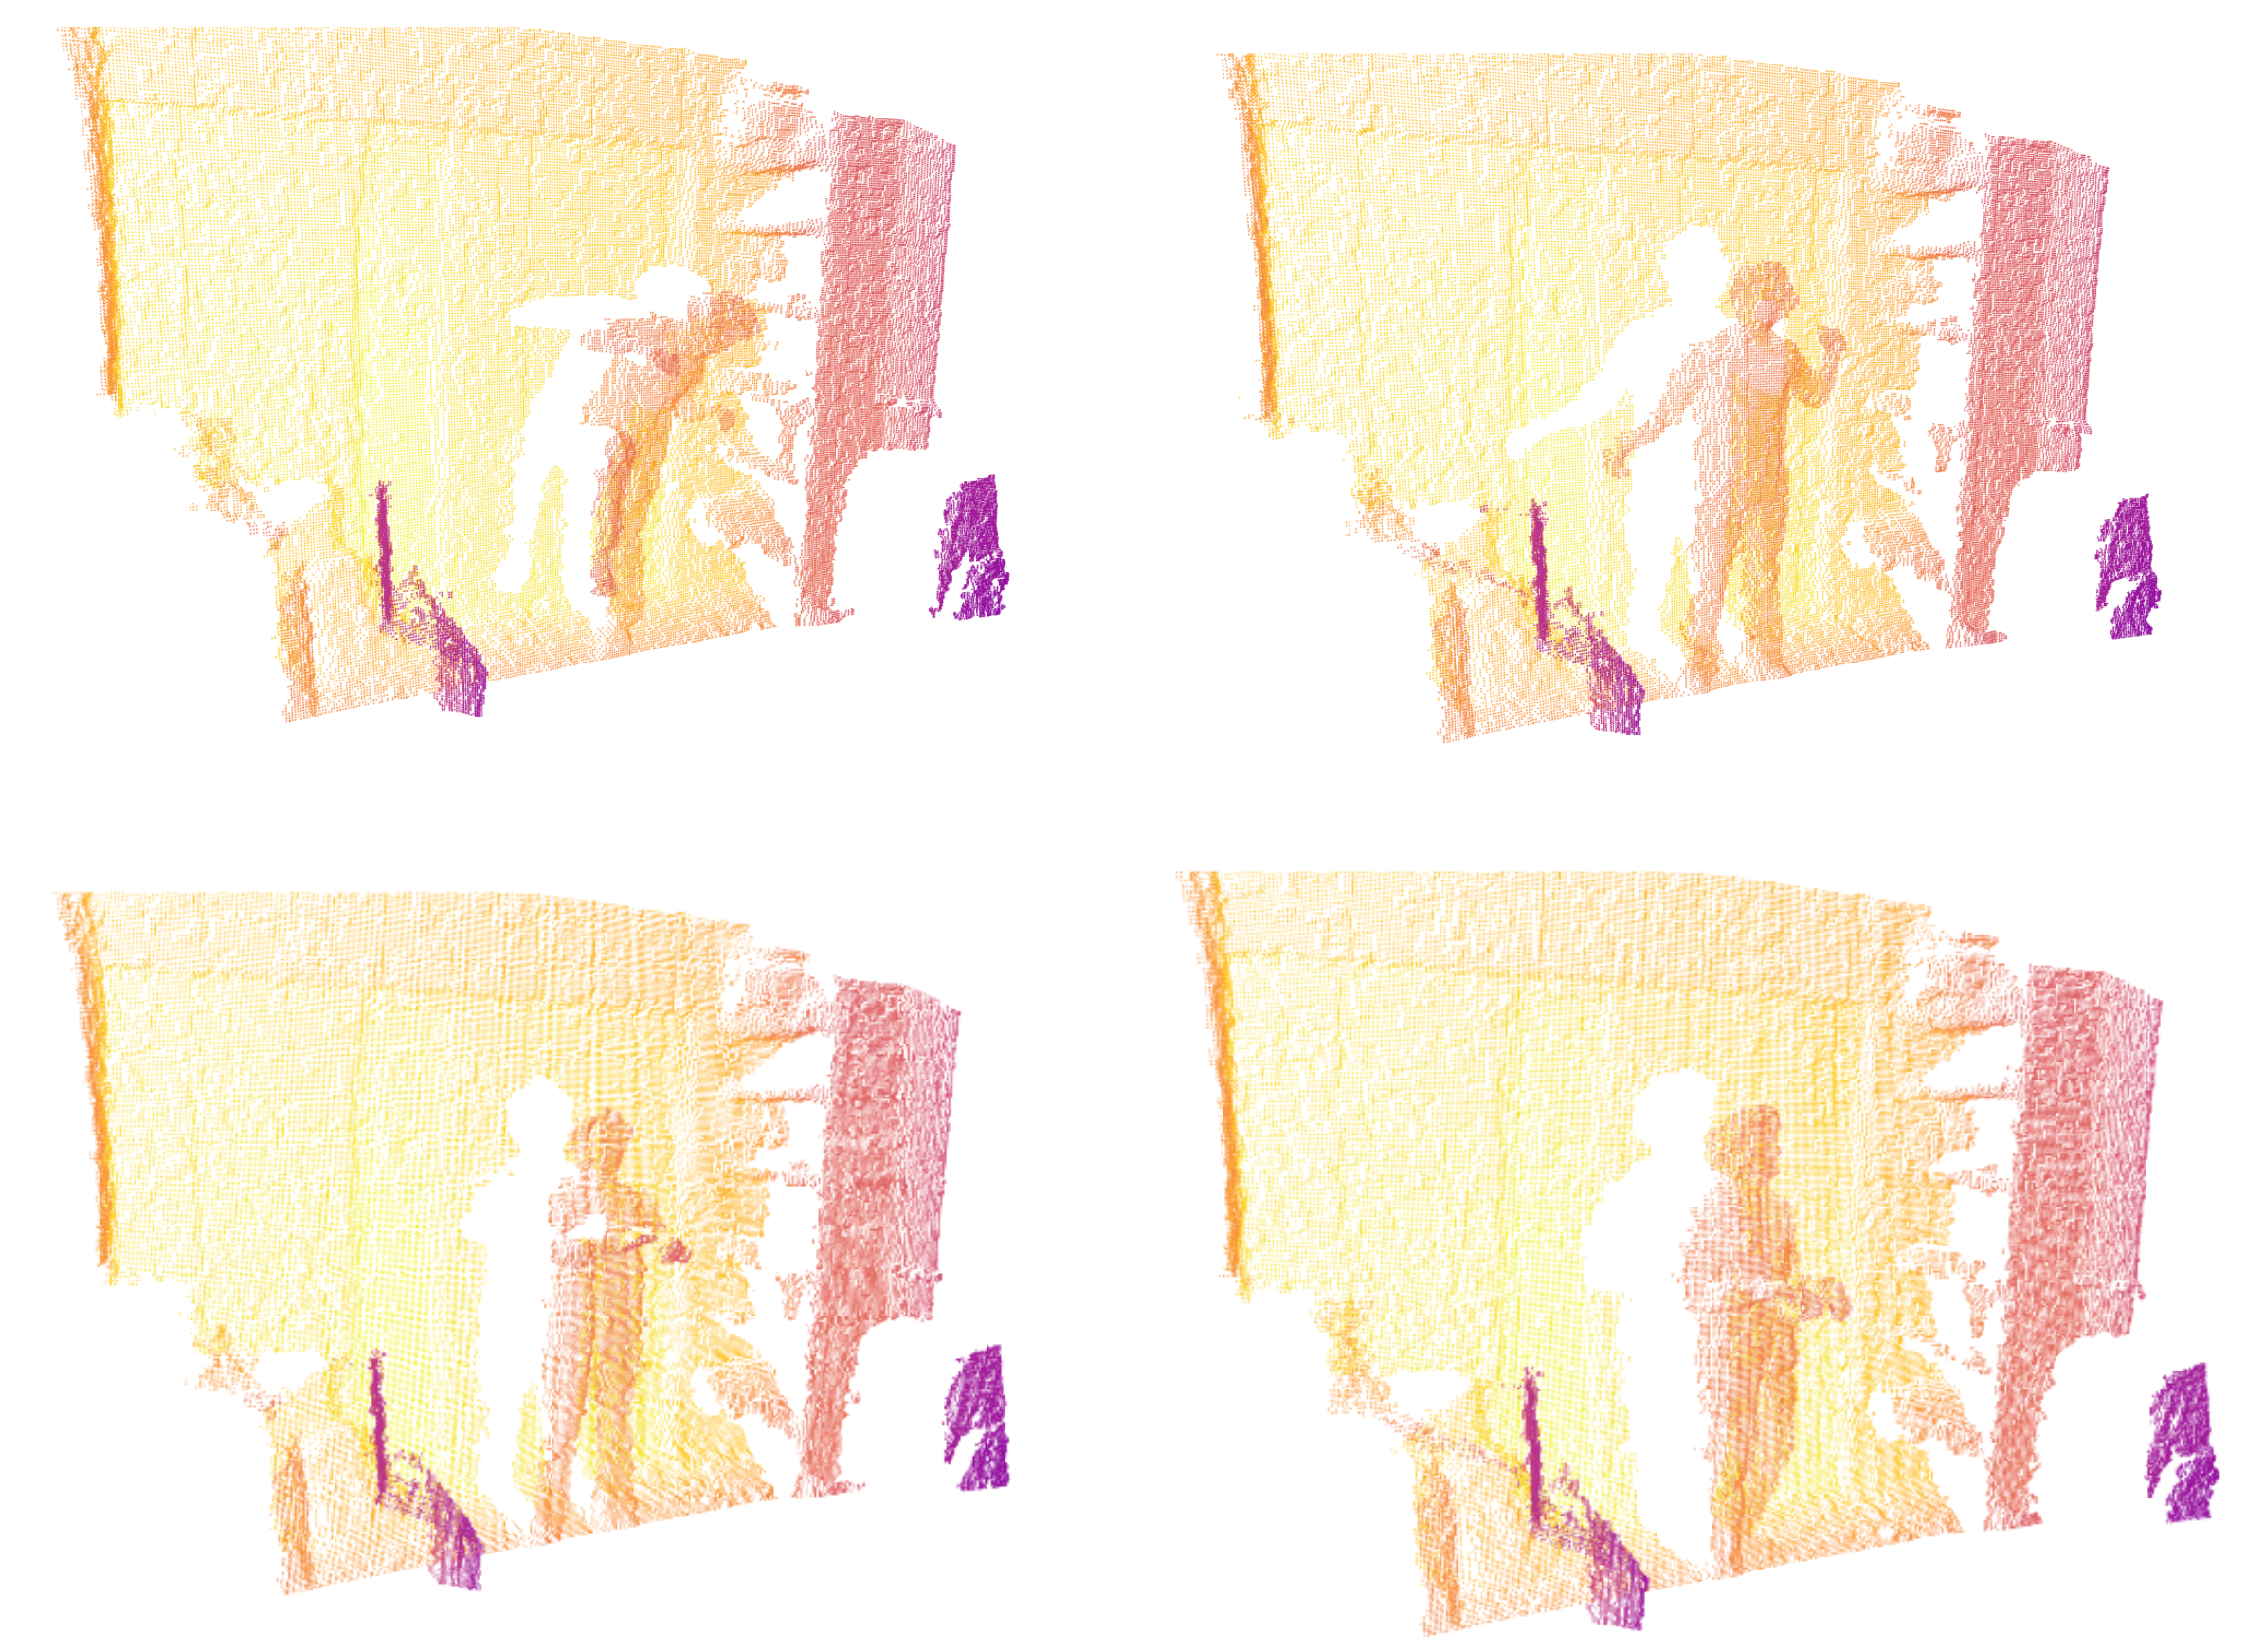
\includegraphics[scale=.17]{Figures/points-with-depth.png}}
    \caption{Four examples of depth images from ITOP dataset. The darker the color the closer it's located to the camera}
    \label{img:dataset-points-with-depth}
\end{figure}

\begin{figure}[htbp]
    \centerline{\includegraphics[scale=.15]{Figures/dataset examples - side view.png}}
    \caption{Four examples of front view subset of ITOP. Upper images are depth representation. Bottom images show human point clouds (blue) with key joints (red)}
    \label{img:dataset-human-examples-front-view}
\end{figure}

\begin{figure}[htbp]
    \centerline{\includegraphics[scale=.15]{Figures/dataset examples - top view.png}}
    \caption{Four examples of top view subset of ITOP. Upper images are depth representation. Bottom images show human point clouds (blue) with key joints (red)}
    \label{img:dataset-human-examples-top-view}
\end{figure}

\begin{figure}[htbp]
    \centerline{\includegraphics[scale=0.8]{Figures/dataset-example-joints.png}}
    \caption{Example of key joints with names from ITOP dataset}
    \label{img:dataset-example-joints}
\end{figure}

\section{Evaluation metric}
\label{evaluation-metric}
Since we are working on the task of the regression, we use mean Average Precision (mAP) as our main metric of model's performance. The ground truths are coordinates of key human joints (denoted as $J$). The output of the regression model is also joints' coordinates of the same size as $J$ (denoted as $\hat{J}$).

To be able to compare our results with other works \parencite{haque_towards_2016,moon_v2v-posenet_2018,guo_towards_2017} we use the same approach of calculation of $AP$ using $10 \ cm$ distance threshold. By this rule (Formula~\ref{eqn:dataset-metric-ap}) the predicted joint is considered correctly detected if the $L_2$ distance to ground truth is equal or less that $10 \ cm$. The resulting $mAP$ is calculated by averaging $AP$ by the number of samples (Formula~\ref{eqn:dataset-metric-map}).

For further convenience we will also apply the plot with $mAP$ values for distances from $0 \ cm$ to $100 \ cm$ (Example in Figure~\ref{img:example-map}).

\begin{equation}
\label{eqn:dataset-metric-ap}
AP(J, \hat{J})=\left\{\begin{array}{ll}
    1, & \lVert J - \hat{J} \rVert <10 \mathrm{~cm} \\
    0, & \text { otherwise }
\end{array}\right.
\end{equation}

\begin{equation}
\label{eqn:dataset-metric-map}
    mAP=\frac{\sum_{i=0}^{M} A P\left(J_{i}, \hat{J_{i}}\right)}{M}
\end{equation}

\begin{figure}[htbp]
    \centerline{\includegraphics[scale=.6]{Figures/example-map.png}}
    \caption{Example of the mAP plot. On the X axis - allowed distance between predicted and ground truth coordinates to be considered as a right detection. On the Y axis - mean Average Precision for given distance. The values for $\textbf{distance} = 10 \ cm$ is highlighted on the plot.}
    \label{img:example-map}
\end{figure} 
\chapter{Experiments}
\label{Experiments}

\section{Capsule network}
\section{Different normalization methods}
\section{Noise}
\label{s:experiment-noise}
\section{Dataset size}
\section{Two stage training}
 
\chapter{Conclusions}

\label{Conclusions}

% from hinton's paper
Now that convolutional neural networks have become the dominant approach to object recognition, it
makes sense to ask whether there are any exponential inefficiencies that may lead to their demise. A
good candidate is the difficulty that convolutional nets have in generalizing to novel viewpoints. The
ability to deal with translation is built in, but for the other dimensions of an affine transformation
we have to chose between replicating feature detectors on a grid that grows exponentially with the
number of dimensions, or increasing the size of the labelled training set in a similarly exponential way.
Capsules (Hinton et al. [2011]) avoid these exponential inefficiencies by converting pixel intensities
8
into vectors of instantiation parameters of recognized fragments and then applying transformation
matrices to the fragments to predict the instantiation parameters of larger fragments. Transformation
matrices that learn to encode the intrinsic spatial relationship between a part and a whole constitute
viewpoint invariant knowledge that automatically generalizes to novel viewpoints.  

%----------------------------------------------------------------------------------------
%	THESIS CONTENT - APPENDICES
%----------------------------------------------------------------------------------------

\appendix % Cue to tell LaTeX that the following "chapters" are Appendices

% Include the appendices of the thesis as separate files from the Appendices folder
% Uncomment the lines as you write the Appendices

% \include{Appendices/AppendixA}
%\include{Appendices/AppendixB}
%\include{Appendices/AppendixC}

%----------------------------------------------------------------------------------------
%	BIBLIOGRAPHY
%----------------------------------------------------------------------------------------

\printbibliography[heading=bibintoc]

%----------------------------------------------------------------------------------------

\end{document}  
